%======================================================================
\chapter{System Architecture}
\label{ch: sysArchitecture}
%======================================================================

%----------------------------------------------------------------------
\section{System Block Diagram}
%----------------------------------------------------------------------
The overall system architecture of this project consists of two subsystems which
are the Mobile Cart and the Remote Target, which is held by the user or
customer, as shown in Fig. \ref{fig:sys_block_diag}. The proposed smart robotic
cart is a wheeled robot that sends and receives radio signals to follow the
remote target which acts as the beacon for the robotic cart system.

\vspace*{12pt}
\noindent
The high-level system block diagram of the proposed robotic cart (prototype) is shown in Fig. \ref{fig:sys_block_diag}. There are three inputs to the proposed cart system. The robotic cart is supplied with power through a battery that is mounted in the chassis of the robotic cart. There will be an on/off switch to allow the system to be powered down when not in use. This will save the battery from being drained by the XBees in the reflector array. The motion of the robotic cart is dependent on the motion of the remote.

\begin{figure}[H]
  \centering
  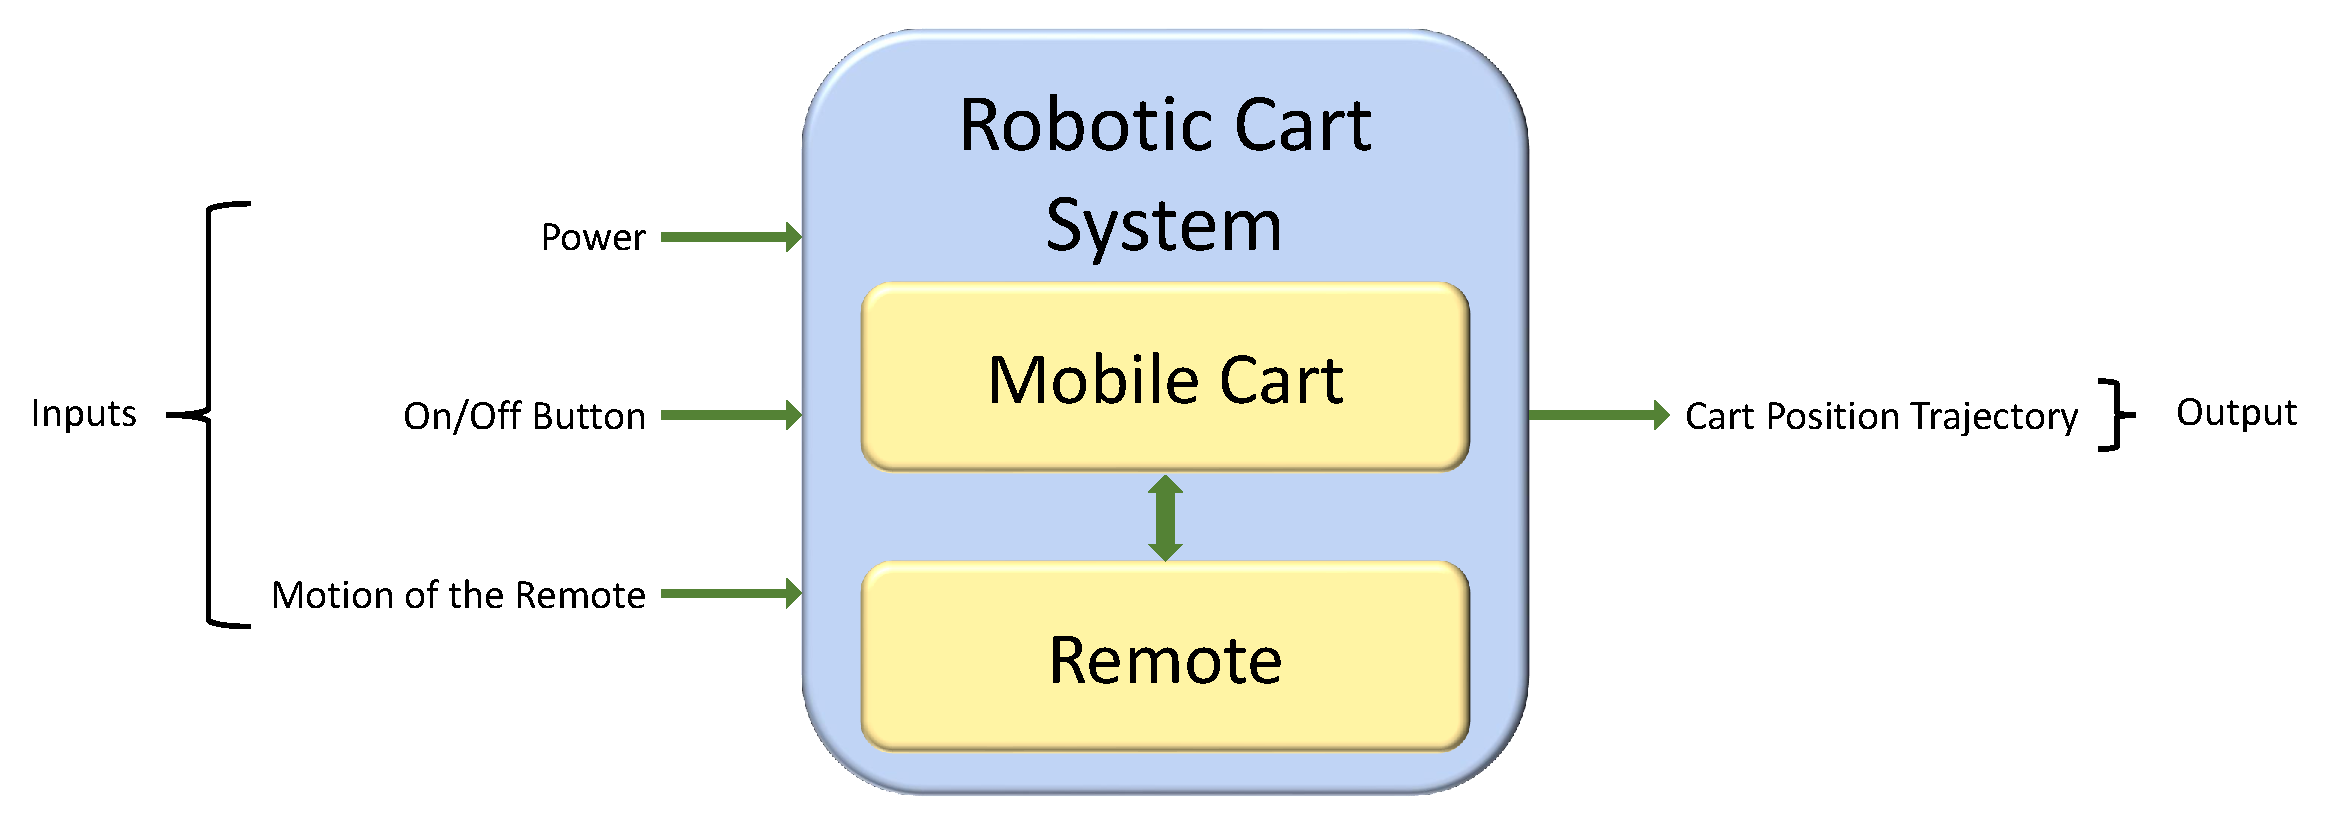
\includegraphics[width=\textwidth]{figs/systemBlockDiagram.pdf}
  \caption{System level block diagram detailing inputs and outputs to the
    robotic cart system.}
	\label{fig:sys_block_diag}
\end{figure}

\vspace*{12pt}
\noindent
The main output of the system is the position trajectory of the robotic cart in its environment. When the user moves with the remote target, the robotic cart is designed to follow the user.



%----------------------------------------------------------------------
\section{Subsystem Block Diagrams}
%----------------------------------------------------------------------
The Mobile Cart and the Remote Target subsystems are two separate operations
within the robotic cart system that run simultaneously. The two subsystems
communicate with one another by relaying radio messages between them. The first
block diagram is of the Remote Target subsystem shown in Fig.
\ref{fig:remote_block_diag}. Of the two subsystems the Remote Target is the
simplest since it only requires an XBee module attached to a 7.4V Li-Po battery
with a voltage regulation circuit since the XBee has a smaller input voltage of
3.3 volts. The two inputs for this system are the battery power and the incoming
RF messages which are passed through the RF transceiver Module and output the
outgoing RF messages.

\begin{figure}[H]
  \centering
  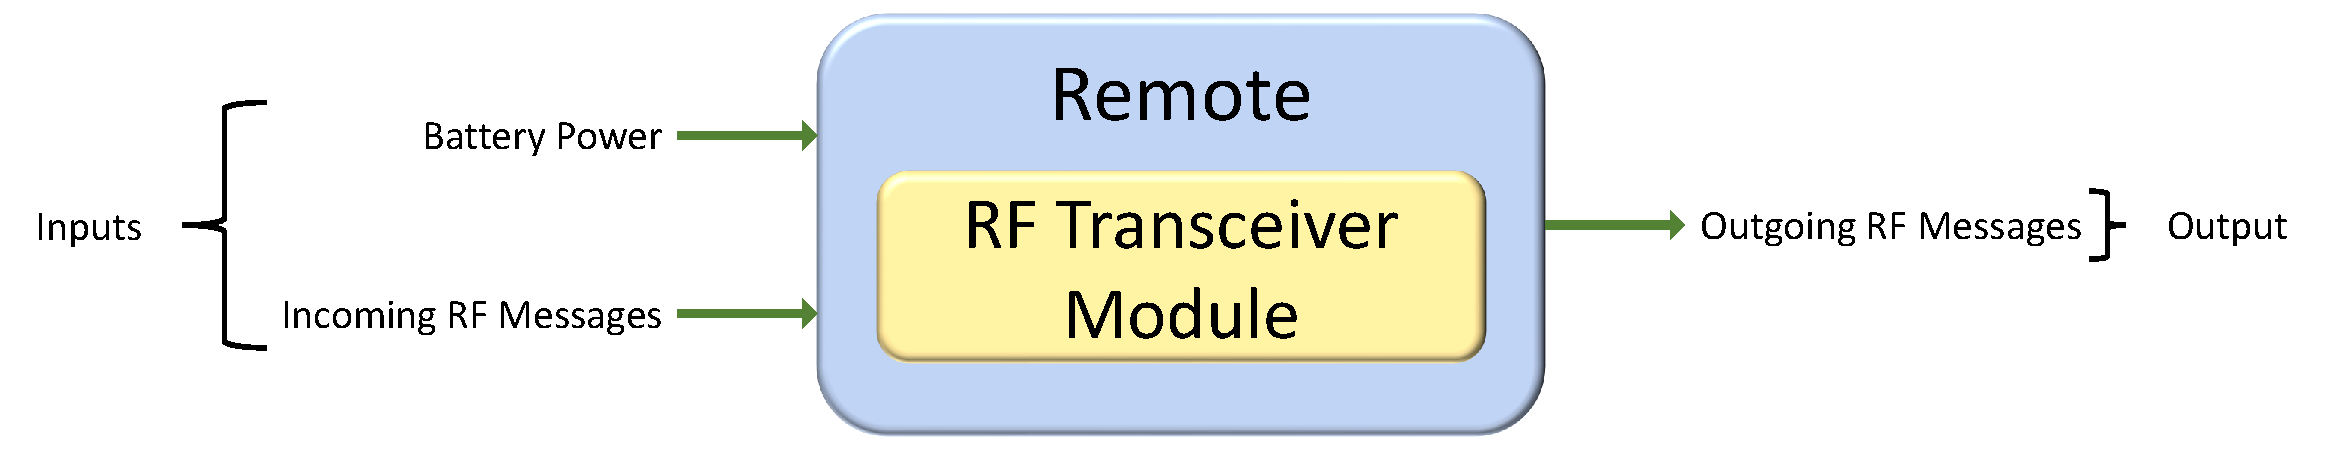
\includegraphics[width=\textwidth]{figs/remoteBlockDiagram.pdf}
  \caption{Remote Target block diagram}
  \label{fig:remote_block_diag}
\end{figure}

\vspace*{12pt}
\noindent
The Mobile Cart subsystem block diagram, shown in Fig.
\ref{fig:mobile_block_diag}, is the most complex of the two subsystems.The cart requires a power source, which will be a 7.4V, 8,000 mAh Li-Po battery since the
Li-Po works well with powering the embedded computer (BeagleBone Blue). The
power to the subsystem will be toggled by an on/off switch located on the
chassis of the robotic cart. The final input to the mobile cart subsystem is the
incoming RF signals. These incoming RF signals are passed to the direction
sensitive RF receivers which output the signals to the dual-direction
multiplexer. The dual-direction multiplexer then takes the four inputs from the
direction sensitive RF receivers and passes one output into the embedded
computer. Once the embedded computer gets these signals it can calculate the
localization and navigation algorithms and pass the information to the DC
motors.

\begin{figure}[H]
  \centering
  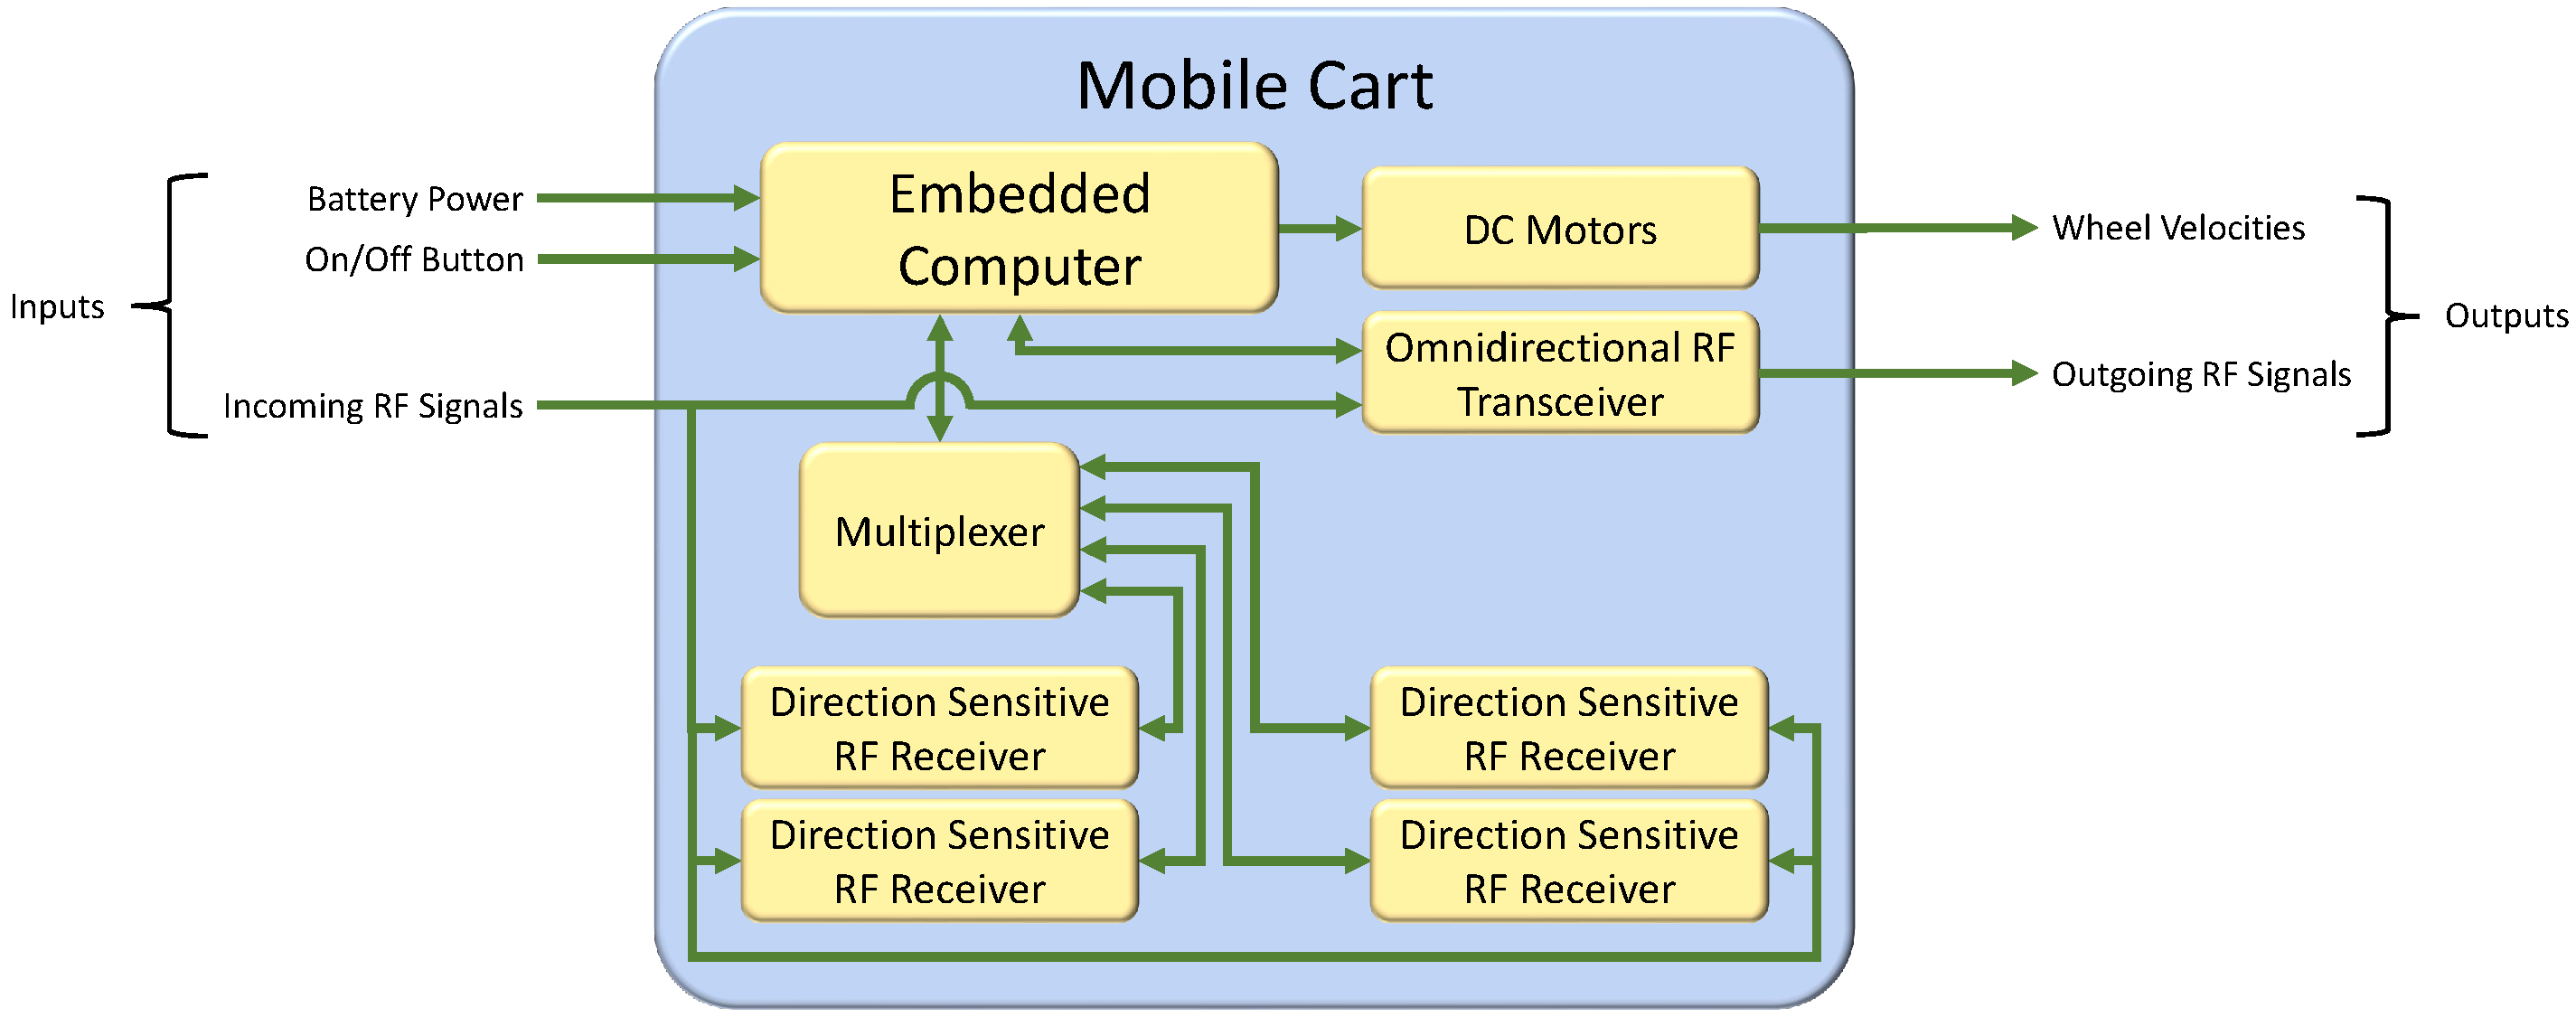
\includegraphics[width=\textwidth]{figs/mobileCartBlockDiagram.pdf}
  \caption{Block diagram showing the subsystem-level components of the proposed robotic cart.}
  \label{fig:mobile_block_diag}
\end{figure}

\vspace*{12pt}
\noindent
There are two outputs of the mobile cart subsystem. The first is the wheel velocities that move the cart and are passed from the DC motors. Lastly, the incoming RF signals are passed to our omnidirectional RF transceiver which outputs the outgoing RF signals.


%----------------------------------------------------------------------
\section{System Components}
\label{sec:System Components}
%----------------------------------------------------------------------

There are several components that are required for the mobile cart system.
Although some of these parts are available in the Bradley University laboratory,
other parts must be purchased. The parts that exist in the lab are listed in
\autoref{tab:Partslablist}. Also, \autoref{tab:Partslist} shows the list of
parts that were purchased. The parts compiled in the lists are the required
parts needed to build two smart robotic cart systems.

\begin{table}[H]
  \centering
  \caption{Parts Available in Laboratory}
  \begin{tabular}{c|c}
      \toprule
      \textbf{Quantity} & \textbf{Parts}\\
      \toprule
      2 & Budget Bot Chassis\\
      4 & 10 uF Ceramic Capacitor\\
      4 & LM1117 Regulator\\
      8 & 9V Batteries\\
      4 & Solderable PCB Boards\\
      3 & XBee USB Adapter\\
      \bottomrule
      %\multicolumn{2}{r|}{\textbf{Total}} & \$ 562.34\\
      %\bottomrule
  \end{tabular}
  %\caption{Parts Available in Laboratory}
  \label{tab:Partslablist}
\end{table}

\begin{table}[H]
  \centering
  \caption{Purchased parts for the Robotic Cart Project}
  \begin{tabular}{c|c|c}
    \toprule
    \textbf{Quantity} & \textbf{Parts} & \textbf{Price}\\
    \toprule
    4 & Pololu 37D Metal Gear motor 4751 & \$ 39.95\\
    12 & XBee S2C Module & \$ 23.10\\
    10 & XBee Adapter Board & \$ 4.99\\
    2 & Twotrees 4 Lead Nema 17 Stepper Motor & \$ 9.99\\
    1 & 4-Pin JST SH Connector - 20 Pack & \$ 7.99\\
    1 & 6-Pin JST SH Connector - 10 Pack & \$ 9.99\\
    1 & Aluminum Foil Tape - 2 in x 5 yd & \$ 6.05\\
    2 & Ovonic 7.4V 8000mAh LiPo Battery & \$ 40.99\\
    4 & Multiplexers & \$ 15.99\\
    \bottomrule
    \multicolumn{2}{r|}{\textbf{Total}} & \$ 562.34\\
    \bottomrule
  \end{tabular}
  %\caption{Purchased parts for the Robotic Cart Project}
  \label{tab:Partslist}
\end{table}

\vspace*{6pt}
\noindent
The main components for this project are the Budget Bot Chassis (Fig.
\ref{fig:budgetBotChassis}), the BeagleBone Blue embedded computer (Fig.
\ref{fig:beagleboneBlue}), and the XBee S2C Modules (Fig. \ref{fig:XBeeModule}).
Another major component is the reflector array that will be used to
directionally receive the RF signals from the remote target that is with the
user, which will be discussed in detail in the next section.

\begin{figure}[H]
  \centering
  \begin{subfigure}[t]{0.32\textwidth}
    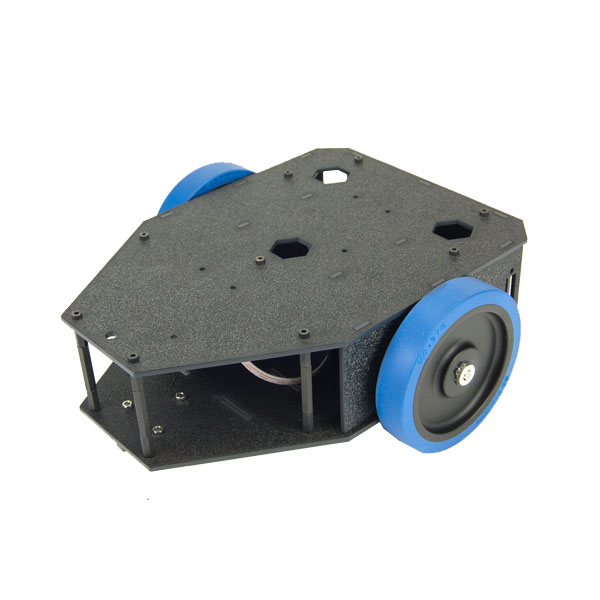
\includegraphics[width=1\textwidth]{figs/img/budgetbot_chassis}
    \captionsetup{width=\textwidth}
    \caption{Budget Bot Chassis}
    \label{fig:budgetBotChassis}
  \end{subfigure}
  \begin{subfigure}[t]{0.32\textwidth}
    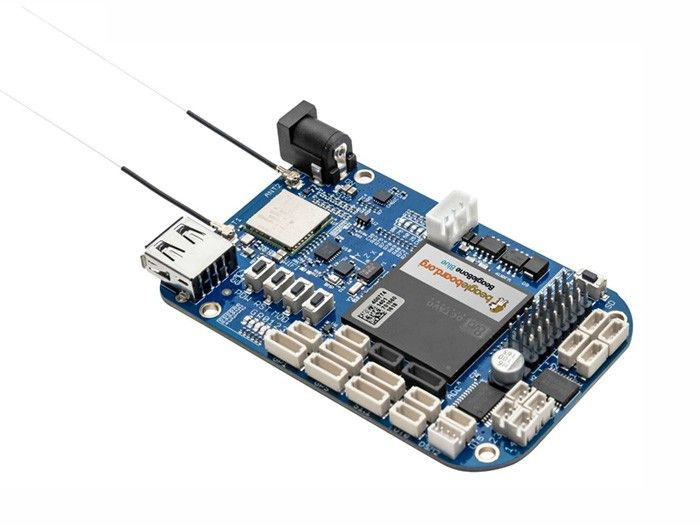
\includegraphics[width=1\textwidth]{figs/img/beaglebone_blue}
    \captionsetup{width=\textwidth}
    \caption{BeagleBone Blue}
    \label{fig:beagleboneBlue}
  \end{subfigure}
  \begin{subfigure}[t]{0.32\textwidth}
    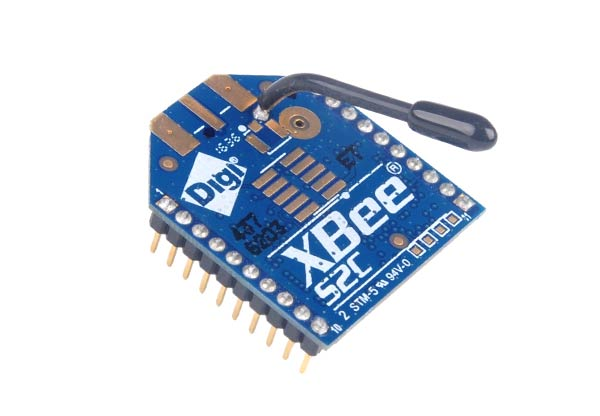
\includegraphics[width=1\textwidth]{figs/img/Xbee-S2C-Module}
    \captionsetup{width=\textwidth}
    \caption{XBee S2C Module}
    \label{fig:XBeeModule}
  \end{subfigure}
  \caption{Main System Components}
\end{figure}

%----------------------------------------------------------------------
\section{Customized Reflector Array}\label{sec:customReflector}
%----------------------------------------------------------------------
The XBee RF modules that were used are omnidirectional. In this project, however, it is desired to have differences in the received signals based on the angle from which the signal is coming. Therefore, one of the major components of this project is the reflector array that enables the XBee modules to be direction sensitive. This section discusses the steps that were taken to construct such a reflector array.

\subsection{Reflector Design}
Two different models of reflector arrays were designed and constructed. The first design was a paraboloidal reflector with the focus on the antenna of the XBee module. The second design was a combination of a paraboloidal shape and a simpler parabolic shape. The motivation for each design will be discussed in sections \ref{subsec:paraboloidalReflector} and \ref{subsec:parabolicReflector}.

\subsubsection{Paraboloidal Reflector}\label{subsec:paraboloidalReflector}
The first design, shown in Fig. \ref{fig:paraboloidalReflector}, uses a reflector with a paraboloidal shape. This shape was selected since all signals entering the reflector parallel to the axis of the reflector will be focused at the focal point of the paraboloid. By mounting the XBee such that the center of the antenna coincides with the focal point of the paraboloid, the signal strength of the signals entering parallel to the axis will be maximized.
\begin{figure}
    \centering
    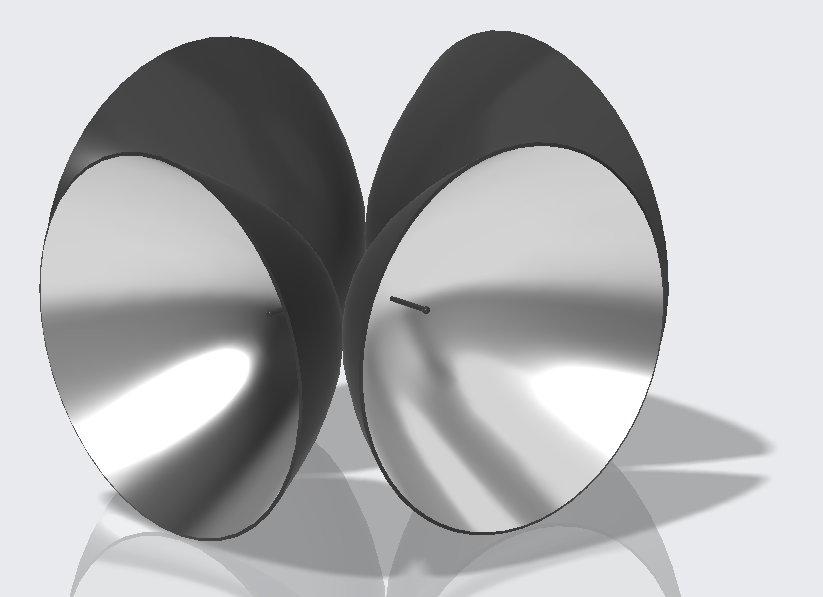
\includegraphics[width=3.5in]{figs/img/paraboloidalReflector.png}
    \caption{Purely Paraboloidal Reflector Array}
    \label{fig:paraboloidalReflector}
\end{figure}

\subsubsection{Combined Parabolic/Paraboloidal Reflector}\label{subsec:parabolicReflector}
The second design, shown in Fig. \ref{fig:parabolicReflector}, is the same on the lower half as the first design. However, the upper half is simply a surface where the horizontal cross-section is a parabola. The purpose for this design is similar to that of the first design, but the parabolic shape on the top will allow stronger detected signal strength of signals coming from above the reflector. Since the remote will be held by a person, it will generally be above the robot. The parabolic/paraboloidal reflector design is intended to allow better reception of signals from above.
\begin{figure}
    \centering
    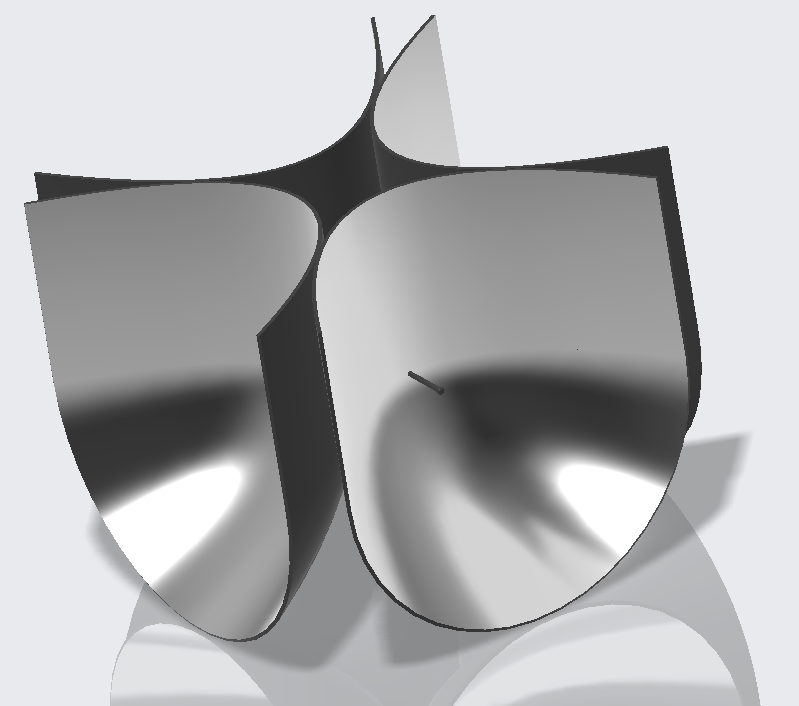
\includegraphics[width=3.5in]{figs/img/parabolicReflector.png}
    \caption{Parabolic/Paraboloidal Reflector Array}
    \label{fig:parabolicReflector}
\end{figure}

\subsection{Reflector Construction}
With the recent advancements in 3D printing technology, it is not difficult to
create an object with a parabolic shape. In this project, the reflector dishes
were created using a 3D printer. The reflector array was designed to be modular,
where the dishes, top plate, and bottom frame were printed separately. After
printing, the dishes were lined with foil tape to provide the reflective surface
to focus the signals onto the antenna of the XBee. A layer of foil tape was also
placed on the top plate to provide a ground plane for the XBee. The parts were
then fastened together using M3 screws and nuts (Fig.
\ref{fig:reflectorConstruction}).
%
\begin{figure}[H]
    \centering
    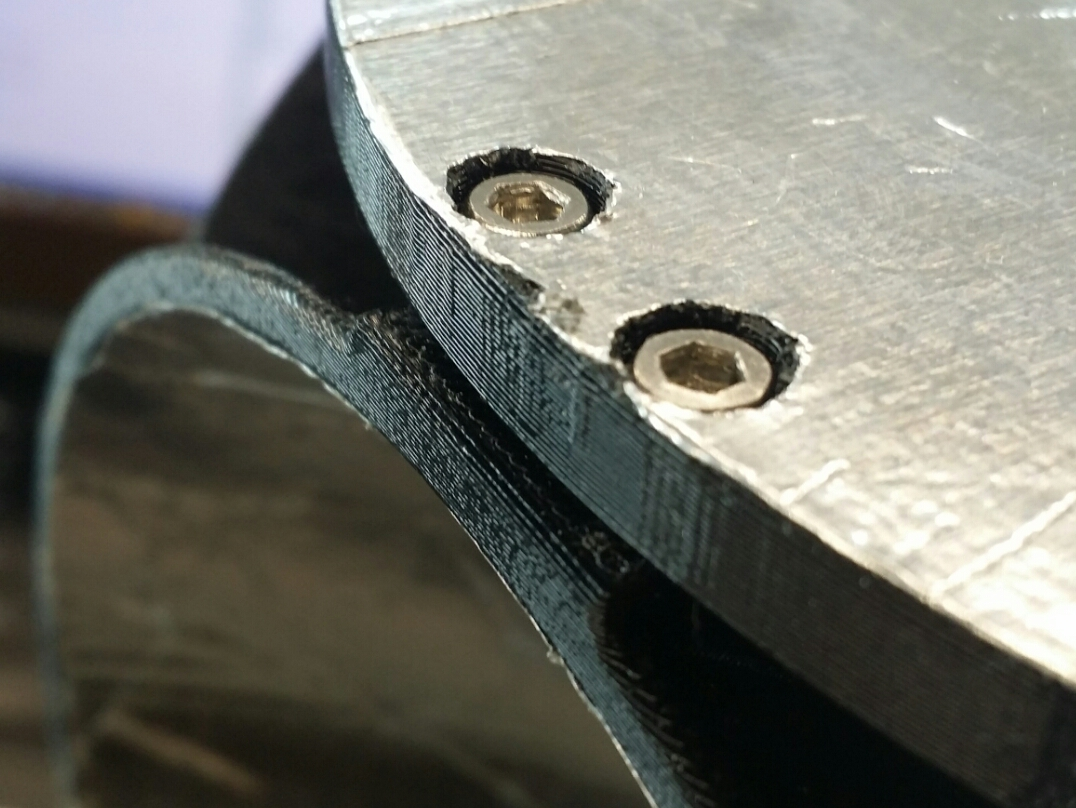
\includegraphics[width=2.5in]{figs/img/reflectorConstruction.jpg}
    \caption{Reflector Construction}
    \label{fig:reflectorConstruction}
\end{figure}

%----------------------------------------------------------------------
\section{Localization and Navigation}\label{sec:locAndNavAlgos}
%----------------------------------------------------------------------

This section illustrates the localization and navigation algorithms for the mobile cart to operate in an indoor/outdoor environment. The proposed robotic cart was modeled as a differential drive mobile robot (DDMR). The direction and distance of the remote relative to the cart are determined using a localization algorithm. This distance and angle are then passed to a navigation algorithm which calculates and applies the wheel speeds to move the robot toward the remote.

\subsection{Robot Model}\label{subsec:robotModel}
The robot used in this project was a differential drive mobile robot, which has
two drive wheels and a caster wheel for balance. The robot turns by applying
different speeds to the left and right wheels. As shown in Fig.
\ref{fig:robotGeometry}, the radius of the wheels is $R$, and the distance
between the wheels is $L$. The pose of the robot is given by the $x$-coordinate
($x$), the $y$-coordinate ($y$), and the orientation, ($\theta$), as shown in
Fig. \ref{fig:robotPose}. %
%
\begin{figure}[H]
    \centering
    \begin{subfigure}{0.3\textwidth}
        \centering
        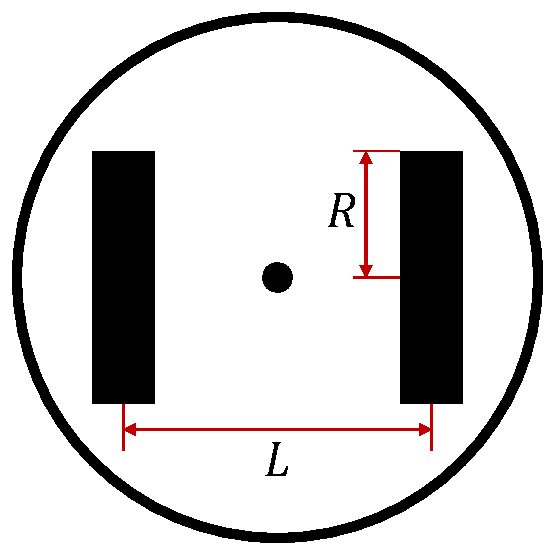
\includegraphics[width=0.7\textwidth]{figs/robotGeometry.pdf}
        \caption{Robot Geometry}
        \label{fig:robotGeometry}
    \end{subfigure}%
    \begin{subfigure}{0.7\textwidth}
        \centering
        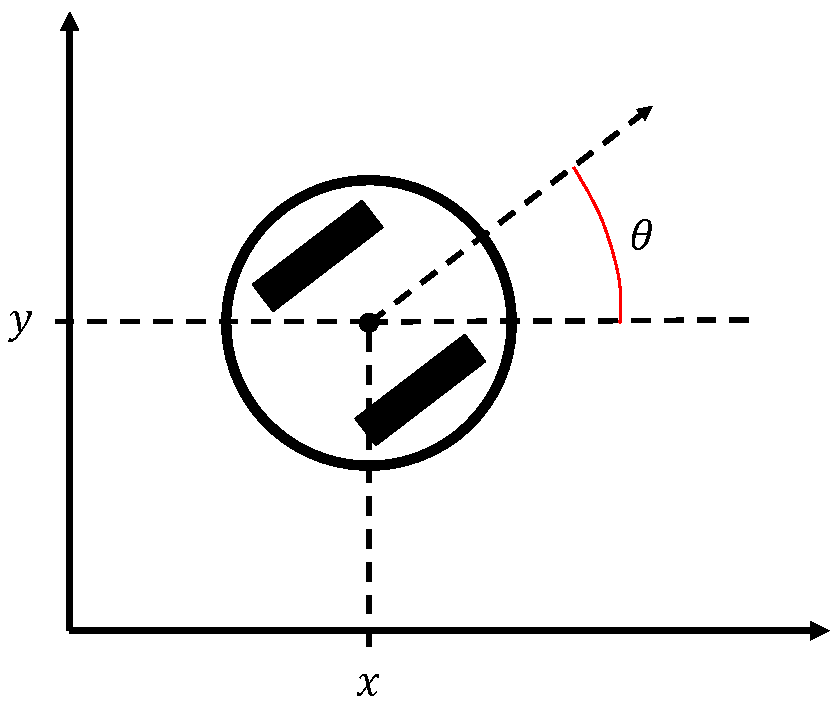
\includegraphics[width=0.7\textwidth]{figs/robotPose.pdf}
        \caption{Robot Pose}
        \label{fig:robotPose}
    \end{subfigure}
    \caption{Robot Model Parameters}
    \label{fig:robotModelParameters}
\end{figure}
%

\vspace*{12pt}
\noindent
Generally the robot is controlled by commanding a linear and angular speed ($v$ and $\omega$, respectively). These speeds must be converted into left and right wheel speeds. The following equations are used to calculate the angular left and right wheel speeds ($\omega_l$ and $\omega_r$, respectively):
$$\omega_l = \left(v - \omega\frac{L}{2}\right)\frac{1}{R}$$
$$\omega_r = \left(v + \omega\frac{L}{2}\right)\frac{1}{R}$$
To control DC motors in this way, the relationship between duty cycle and angular speed must be determined. Then the duty cycles to apply to the wheels can be calculated for the commanded $v$ and $\omega$.

\subsection{Localization Algorithm}
The localization algorithm is used to estimate the position of the remote with respect to the robot's local coordinate system. First the omnidirectional transceiver on top of the reflectors sends a signal strength request to the remote. The remote then replies with a message containing the strength of the signal it just received. This reply is detected by the receivers inside the reflectors as well as the omnidirectional transceiver. The strength detected by each of the directional receivers and the strength contained in the reply are then recorded. At this point, the entire reflector array is rotated 9\textdegree, and this process is repeated. The robot continues taking measurements in this way until the reflectors have been rotated one quarter turn. Since there are four reflectors at 90\textdegree to each other, a strength measurement has been recorded for every 9\textdegree increment around the robot. The angle of the remote is then estimated as the direction from which the strongest signal was received. The distance to the remote is calculated using the free-space path loss formula. The direction of reflector rotation is then reversed since the wires connecting the RF modules in the reflectors prevent the reflector from freely spinning. A flowchart of this algorithm is shown in Fig. \ref{fig:localizationAlgoFlowchart}.
\begin{figure}[H]
    \centering
    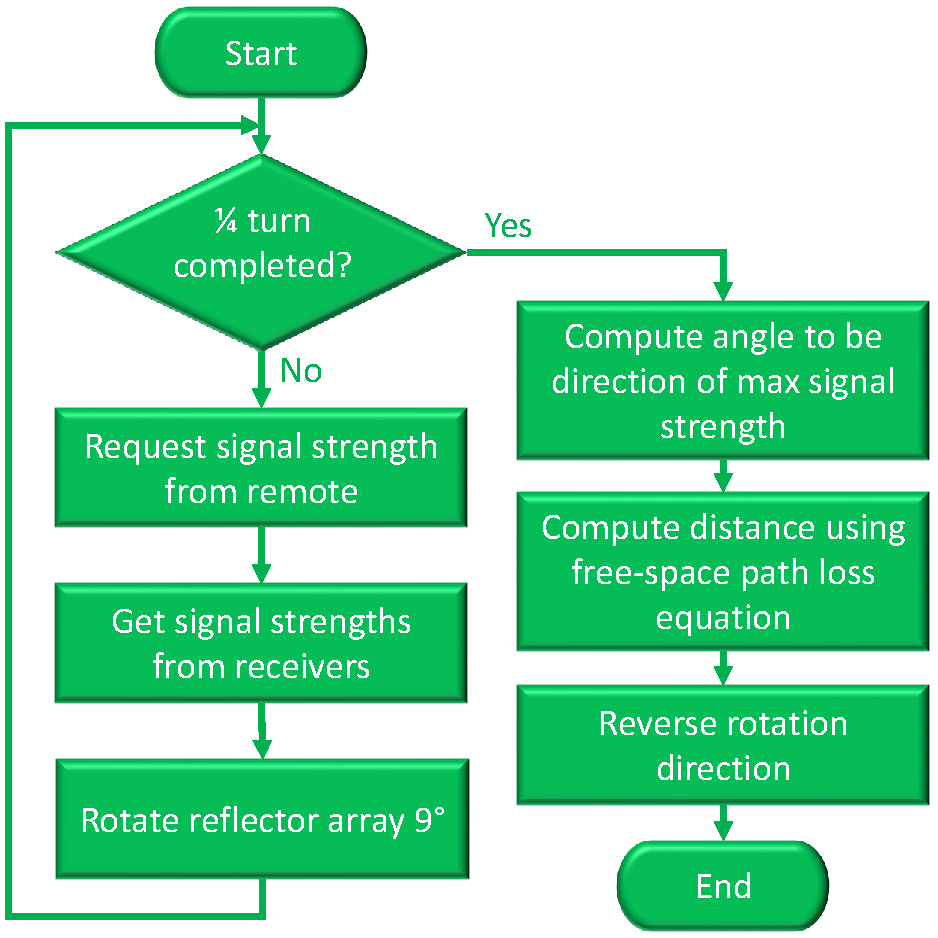
\includegraphics[width=3.5in]{figs/localizationAlgorithmFlowchart.pdf}
    \caption{Flowchart of Localization Algorithm}
    \label{fig:localizationAlgoFlowchart}
\end{figure}

\subsection{Navigation Algorithm}\label{subsec:navAlgo}
The navigation algorithm is used to drive the robot toward the remote. The inputs to the navigation algorithm are the angle to the remote ($\theta_r$) and the distance to the remote ($d_r$). A target point is then calculated as the point that is in the same direction as the remote, but closer to the robot by a fixed following distance ($d_{follow}$), as shown in Fig. \ref{fig:navAlgoDiagram}. The distance to the target point is calculated as $d_{tgt} = d_r - d_{follow}$, and the angle to the target point is $\theta_{tgt} = \theta_r$. The linear and angular speeds of the robot ($v$ and $\omega$, respectively) are then calculated using proportional control by the following equations:
$$v = K_vd_{tgt}$$
$$\omega = K_\omega\theta_{tgt}$$
The appropriate duty cycles are then calculated as specified in section \ref{subsec:robotModel} and applied to the wheel motors.
\begin{figure}[H]
    \centering
    \begin{subfigure}{0.45\textwidth}
        \centering
        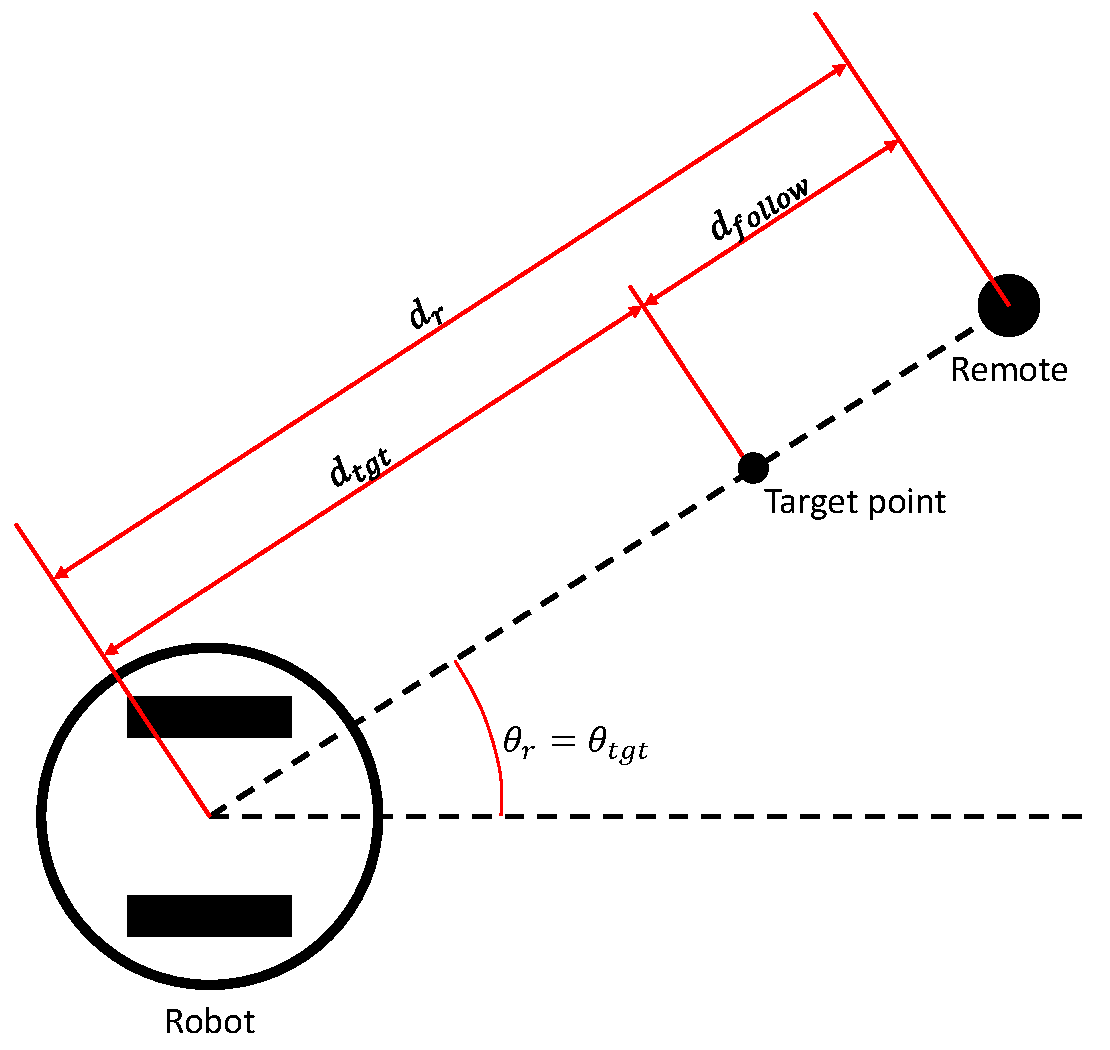
\includegraphics[width=0.95\textwidth]{figs/navigationAlgorithmDiagram.pdf}
        \caption{Target Point Diagram}
        \label{fig:navAlgoDiagram}
    \end{subfigure}%
    \begin{subfigure}{0.55\textwidth}
        \centering
        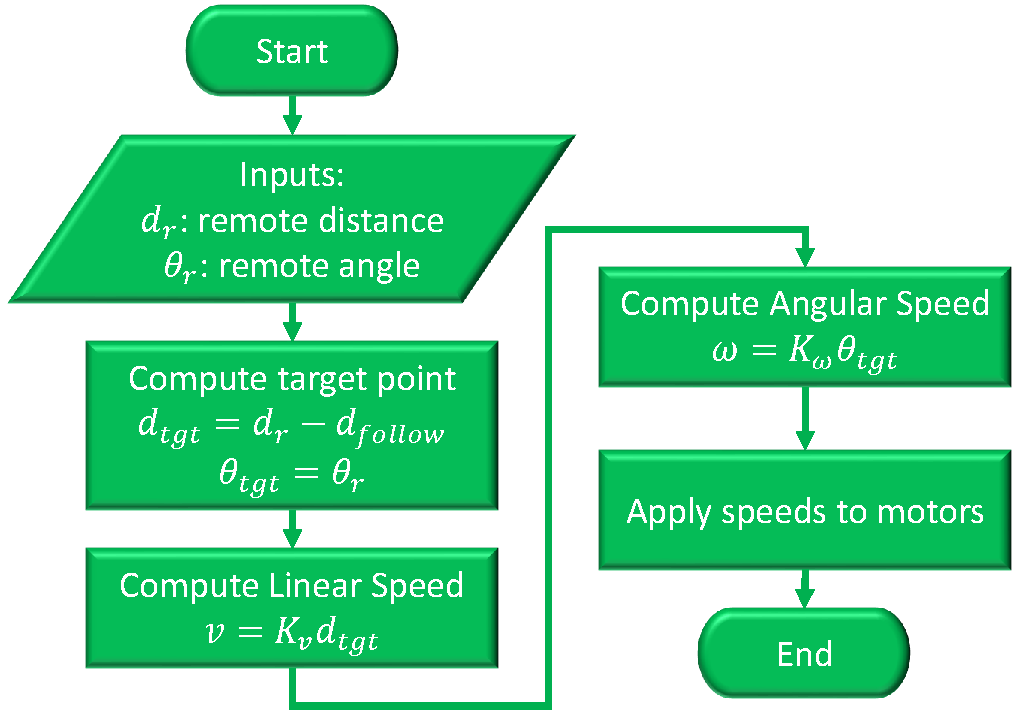
\includegraphics[width=0.95\textwidth]{figs/navigationAlgorithmFlowchart.pdf}
        \caption{Flowchart}
        \label{fig:navAlgoFlowchart}
    \end{subfigure}
    \caption{Navigation Algorithm Details}
    \label{fig:navAlgoDetails}
\end{figure}

%%% Local Variables:
%%% mode: latex
%%% TeX-master: "../finalReport"
%%% End:
